\documentclass[letterpaper]{article}

\usepackage{ifthen}
\usepackage{xparse}
\usepackage{enumitem}
\usepackage[utf8]{inputenc}
\usepackage{amsmath}
\usepackage{amssymb}
\usepackage{stmaryrd}
\usepackage{amsthm}
\usepackage{mathtools}
\usepackage{proof}
\usepackage{colonequals}
\usepackage{comment}
\usepackage{textcomp}
\usepackage[us]{optional}
\usepackage{color}
\usepackage{url}
\usepackage{verbatim}
\usepackage{graphics}
\usepackage{mathpartir}
\usepackage{tikz}
\usepackage{todonotes}

% these two are used to create the wavy division sign
\usepackage{stackengine}
\usepackage{scalerel}

\usepackage{hyperref}
\usepackage[nameinlink, capitalise]{cleveref}

\usepackage{array}


%% Beamer defines a range of its own theorems
\ifx\beamer\undefined

\theoremstyle{plain}
\newtheorem{theorem}{Theorem}[section]
\newtheorem{lemma}[theorem]{Lemma}
\newtheorem{corollary}[theorem]{Corollary}

\theoremstyle{definition}
\newtheorem*{remark}{Remark}
\newtheorem*{notation}{Notation}
\newtheorem{definition}{Definition}
\newtheorem{conjecture}{Conjecture}
\newtheorem{example}{Example}

\else 
  %% Intentionally left blank
\fi

\makeatletter
\newcommand\xlabel[2][]{\phantomsection\def\@currentlabelname{#1}\label{#2}}
\makeatother

\newenvironment{rules}[1][{}]{\begin{mathpar}}{\end{mathpar}}

%% This puts the name on the top
\NewDocumentCommand{\defrule}{o o m m}{
  \inferrule*[lab=\IfNoValueTF{#1}{}{\textsc{[#1]}}]
  { #3 }
  { #4 }
  \IfNoValueTF{#2}{}{\xlabel[#1]{\ifdefined\InApx{apx:}\else\fi#2}}
}


\NewDocumentCommand{\ruleref}{m}{{[\textsc{\nameref{#1}}]}}


\usepackage[abt]{pl-syntax}
\usepackage{pl-judgments}

%% \xMapsto command
% \usepackage{mathtools}
\usepackage{stmaryrd}

\makeatletter
\newcommand{\xMapsto}[2][]{\ext@arrow 0599{\Mapstofill@}{#1}{#2}}
\def\Mapstofill@{\arrowfill@{\Mapstochar\Relbar}\Relbar\Rightarrow}
\makeatother

%% Instructor-only remarks. These remarks requires the benefit of the hind sight to understand
%% (or foreshadowing) future content so it doesn't make sense to put it in the file
%% Define \isstudentcopy to generate the student version
\definecolor{iremarkcolor}{rgb}{0.0, 0.0, 0.5}
\NewDocumentEnvironment{iremark}{ +b }
{ \ifthenelse{\isundefined{\isstudentcopy}}{
    \begingroup
    \color{iremarkcolor}
    \begin{remark}
    #1
    \end{remark}
    \endgroup
  }{
  }
}{ }

\newcommand{\inlremark}[1]{\ifthenelse{\isundefined{\isstudentcopy}}{\begingroup\color{iremarkcolor}(#1)\endgroup}{}}
\newcommand{\PFPL}{\textbf{\textsf{PFPL}}}

\makeatletter

\NewDocumentCommand{\fstEx}{s O{\tau_1} O{\tau_2} m}{\IfBooleanTF{#1}{\projEx*<1>[#2][#3]{#4}}{\projEx<1>[#2][#3]{#4}}}
\NewDocumentCommand{\sndEx}{s O{\tau_1} O{\tau_2} m}{\IfBooleanTF{#1}{\projEx*<2>[#2][#3]{#4}}{\projEx<2>[#2][#3]{#4}}}

\NewDocumentCommand{\hatM}{}{\hat{M}}

\NewDocumentCommand{\Iff}{}{\,\mathrm{iff}\,}
\NewDocumentCommand{\limp}{}{\supset}

\NewDocumentCommand{\HT}{O{A}}{\mathsf{HT}_{#1}}


\makeatother



\usepackage{tikz}
\usetikzlibrary{automata,positioning}

\usepackage{todonotes}

\newcommand{\gmhat}[1]{\ensuremath{\widehat{\gamma}(#1)}}

\newcommand{\De}[0]{\Delta}
\newcommand{\Ga}[0]{\Gamma}
\newcommand{\ga}[0]{\gamma}

\newcommand{\whBetaReducesTo}[0]{\mapsto_\beta}
\newcommand{\betaReducesTo}[0]{\to_\beta}

\newcommand{\whBetaNormal}[1]{#1\ \mathsf{whnorm}_\beta}
\newcommand{\betaNormal}[1]{#1\ \mathsf{norm}_\beta}

\newcommand{\betaNorm}[1]{\mathsf{norm}_\beta(#1)}

\newcommand{\HN}[3]{\mathsf{HN}^{#1}_{#2}(#3)}
\newcommand{\NN}[3]{\mathsf{NN}^{#1}_{#2}(#3)}

\title{15-791 ATPL \\ Week 2 Notes}
\author{Hemant Gouni and Josh Grosso}
\date{\today}

\begin{document}

\maketitle

\section{Natural Numbers and Co-Natural Numbers}

\subsection{Co-Natural Numbers}

We extend our language from the previous lecture with a simple coinductive
type, in particular conatural numbers. The grammar is given by

$$
A \coloncolonequals \cdots \mid \conatTy
$$
$$
M \coloncolonequals \cdots \mid \outEx*{M} \mid \genEx*{M}{x}{N}
$$

\noindent
The statics is given in a standard way:

\begin{mathpar}
\defrule[T-Conat-I][sta:gen]
    {\Gamma \entails{\isOfTp{M}{A}} \\ \Gamma, \isOfTp{x}{A} \entails{\isOfTp{N}{\sumTy*{\unitTy*}{A}}}}
    {\Gamma \entails{\isOfTp{\genEx*{M}{x}{N}}{\conatTy}}}

\defrule[T-Conat-E][sta:out]
    {\Gamma \entails{\isOfTp{M}{\conatTy}}}
    {\Gamma \entails{\isOfTp{\outEx*{M}}{\sumTy*{\unitTy*}{\conatTy}}}}
\end{mathpar}

\noindent
Along with a call-by-name transition system for the dynamics:

\begin{mathpar}
\defrule[V-Gen][dyn:gen-val]
    {}
    {\isVal{\genEx*{M}{x}{N}}}

\defrule[D-Pred-C][dyn:pred-c]
    {M \stepsTo{} M'}
    {\outEx*{M} \stepsTo{} \outEx*{M'}}

\defrule[D-Pred-1][dyn:pred-1]
    {}
    {\outEx*{\genEx*{M}{x}{N}} \mapsto \xcaseEx*{\Sub{M}{x}{N}}{\_}{\injEx*<1>{\unitEx*}}{y}{\injEx*<2>{\genEx*{y}{x}{N}}}}
\end{mathpar}

\subsection{Co-Naturals as State Machines}

\noindent
The semantics of $\genEx*{M}{x}{N}$ bears explanation. Conatural numbers can be
understood in terms of \textit{state machines}. Describing $\genEx*{M}{x}{N}$
in the language of state machines:

\begin{enumerate}
    \item $M$ is the prior state
    \item $N$ is the state transformer, determining the next state
    \item $\outEx*{}$ induces a transition to the next state
\end{enumerate}

\begin{figure}[h]
\begin{center}
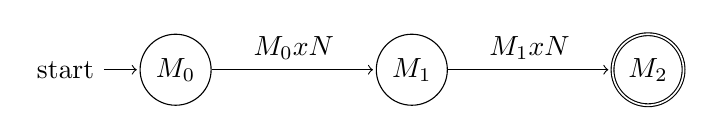
\begin{tikzpicture}[shorten >=1pt,node distance=3cm,on grid,auto]
    \node[state,initial] (M_0) {$M_0$};
    \node[state] (M_1) [right=of M_0] {$M_1$};
    \node[state,accepting](M_2) [right=of M_1] {$M_2$};
      \path[->]
      (M_0) edge node {$\Sub{M_0}{x}{N}$} (M_1)
      (M_1) edge node {$\Sub{M_1}{x}{N}$} (M_2);
\end{tikzpicture}
\end{center}
\caption{A simple state machine}
\label{fig:state-machine-1}
\end{figure}

For a concrete example, consider the machine in \ref{fig:state-machine-1}.
$M_0$ is the initial state. We can think about invoking
$\outEx*{\genEx*{M_0}{x}{N}}$ to get to the next state $M_1$. $M_1$ is
calculated by evaluating $\Sub{M_0}{x}{N}$. In this example $M_1$ is not a
(doubly-circled) end state--- in other words, it's not of unit type--- so by
\ruleref{dyn:pred-1} we get a new value $\genEx*{M_1}{x}{N}$. Observe that in
order to transition to the next state, we must invoke
$\outEx*{\genEx*{M_1}{x}{N}}$ once more. $\genEx*{M_1}{x}{N}$ by itself does
not compute further.

The next transition operates similarly, with the exception of resulting in a
unit value. In this case, we can no longer induce any further transitions
because we're not left with a \texttt{gen} form.

\begin{figure}[h]
\begin{center}
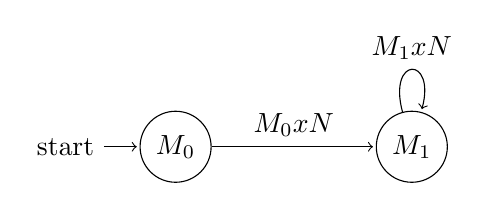
\begin{tikzpicture}[shorten >=1pt,node distance=3cm,on grid,auto]
    \node[state,initial] (M_0) {$M_0$};
    \node[state] (M_1) [right=of M_0] {$M_1$};
      \path[->]
      (M_0) edge node {$\Sub{M_0}{x}{N}$} (M_1)
      (M_1) edge [loop above] node {$\Sub{M_1}{x}{N}$} ();
\end{tikzpicture}
\end{center}
\caption{A state machine without an end state}
\label{fig:state-machine-2}
\end{figure}

It is also worth noting that, as shown in \ref{fig:state-machine-2}, the state
machine represented by a \texttt{conat} \textit{need not have an end state}. In
this instance, $\outEx*{\genEx*{M_1}{x}{N}}$ always evaluates to
$\genEx*{M_1}{x}{N}$--- never to $\unitEx*$. This is not a problem for
termination because, again, a $\genEx*{M_1}{x}{N}$ is inert until `kicked' by
using \texttt{out} on it.

\subsection{Termination for Co-Natural Numbers}

We can proceed with the proof of hereditary termination for co-natural numbers.

\begin{definition}[Hereditary termination for $\conatTy$]
    Define $\HT[\conatTy](M)$ on closed terms $M$ of type $\conatTy$ such that
    one of the following holds:
    \begin{enumerate}
        \item $\outEx*{M} \evalsTo \injEx*<1>{\unitEx*}$.
        \item $\outEx*{M} \evalsTo \injEx*<2>{M'}$ and $\HT[\conatTy](M')$
    \end{enumerate}
\end{definition}

Another way to state this is that $\HT[\conatTy](M)$ is the \textit{weakest}
(or \textit{largest}, when viewed as a set) property $\mathcal{P}$ on closed
terms $\isOfTp{M}{\conatTy}$ such that if $\mathcal{P}(M)$, then either:

\begin{enumerate}
    \item $\outEx*{M} \evalsTo \injEx*<1>{\unitEx*}$
    \item $\outEx*{M} \evalsTo \injEx*<2>{M'}$ and $\mathcal{P}(M')$
\end{enumerate}

Observe this is dualized compared to the case for natural numbers, where having
the analogous properties implied $\mathcal{P}(M)$--- rather than
$\mathcal{P}(M)$ implying these properties. This mirrors the structure of
working (inductively) with natural numbers, versus working (coinductively) with
co-natural numbers.

In order to have a property of natural numbers, we must
evaluate it to know which case we're in, $\zeroEx*$ or $\succEx*{M'}$, and show
the property for it. In contrast, when we use $\outEx*$ on a $\conatTy$
satisfying the property and evaluate the resulting expression, we get something
back that satisfies the necessary properties, but we do not know precisely
which case does so.

% Intuitively, the requirement for $\HT[\conatTy](M)$ to be the $weakest$ such
% property arises from the fact that coinduction maps \textit{out}-- it
% represents a \textit{post fixed-point}. So we must find the \textit{greatest}
% post fixed-point (necessary property is consistency?) in order to reason about
% coinductive types.

\begin{theorem}[Fundamental Theorem]
If $\Gamma \entails{\isOfTp{M}{A}}$ then $\Gamma \gg M \in A$.
\end{theorem}

\begin{proof}
    Proceed by induction on a derivation of $\isOfTp{M}{A}$.
    \begin{enumerate}
        \item [\ruleref{sta:out}]
            Want to show if $\Gamma
            \entails{\isOfTp{\outEx*{M}}{\sumTy*{\unitTy*}{\conatTy}}}$ then
            $\Gamma \gg \outEx*{M} \in \sumTy*{\unitTy*}{\conatTy}$.
            We have by inversion that $\Gamma \entails{\isOfTp{M}{\conatTy}}$.
            Then by induction we know $\Gamma \gg M \in \conatTy$.
            We now want to show that $\HT[\sumTy*{\unitTy*}{\conatTy}](\gmhat{\outEx*{M}})$.
            We have to show that either $\gmhat{\outEx*{M}} \evalsTo
            \injEx*<1>{\unitEx*}$ or $\gmhat{\outEx*{M}} \evalsTo
            \injEx*<2>{M'}$ and $\HT[\conatTy](M')$.
            This is exactly the definition of $\HT[\conatTy](\gmhat{M})$, which
            we have by induction, so we're done.
        \item [\ruleref{sta:gen}]
            Want to show if $\Gamma
            \entails{\isOfTp{\genEx*{M}{x}{N}}{\conatTy}}$ then $\Gamma \gg
            \genEx*{M}{x}{N} \in \conatTy$.

            For convenience, define $G(-) \triangleq \genEx*{-}{x}{\gmhat{N}}$.
            Additionally, define $M_0 \triangleq \gmhat{M}$.
            We begin by reasoning about some $P$ which is consistent against
            $\HT[\conatTy]$.
            We'll show that this $P$ holds, and because $P$ implies
            $\HT[\conatTy]$ (by its consistency against the latter), we'll have
            the property. Let's list the properties we'd like out of $P$.
            For all $\isOfTp{M}{\conatTy}$:

            \begin{enumerate}
                \item if $P(M)$ then
                    $(\sumTy*{\unitTy*}{P})
                     \footnote{$(\sumTy*{\unitTy*}{P})(\outEx*{M})$ is
                     equivalent to evaluating and casing on $\outEx*{M}$, then
                     returning the left injection unmodified, or the right
                     injection with $P$ applied to it.}
                     (\outEx*{M})$
                     \label{itm:conat-p1}
                \item $P(G(M_0))$ \label{itm:conat-p2}
            \end{enumerate}

            % larger = weaker because it's easier to find an element of the set
            Any $P$ satisfying \ref{itm:conat-p1} is consistent against
            $\HT[\conatTy]$, therefore implying it, because $\HT[\conatTy]$ is
            defined to be the \textit{largest} such property-- so it contains
            $P$ (alternatively, it's the \textit{weakest} such property-- so
            it's implied by $P$). \ref{itm:conat-p2} will be important as the
            coinductive `base case', letting us get a foothold in the initial
            state so we can show the property coinductively for future states.
            Take the following to be the definition of $P$; we will show its
            consistency later:

            \begin{definition}[Definition of $P$]
                Assume for all $M : A$ we have $\HT[A](M)$.
                Define $P(M) \triangleq M \evalsTo G(M')$ for some $\HT[A](M')$.
            \end{definition}

            % NOTE [Harrison]: This doesn't work!

            % To show that this satisfies consistency with $\HT[\conatTy]$, show
            % that if $P(X)$ then $(\sumTy*{\unitTy*}{P})(\outEx*{X})$.

            % \begin{proof}
            %     Assume $X \evalsTo G(M)$ with $\HT[A](M)$.
            %     Then in the first case:
            %     \begin{align*}
            %         \outEx*{X} \evalsTo&\, \outEx*{G(M)}\\
            %                    \evalsTo&\, (\sumTy*{\unitTy*}{G})(\Sub{M}{x}{N})\\
            %                    \evalsTo&\, \injEx*<1>{\unitEx*}
            %     \end{align*}
            %     Where consistency is immediate from the first case of
            %     $\HT[\conatTy]$. Or in the second case:
            %     \begin{align*}
            %         \outEx*{X} \evalsTo&\, \outEx*{G(M)}\\
            %                    \evalsTo&\, (\sumTy*{\unitTy*}{G})(\Sub{M}{x}{N})\\
            %                    \evalsTo&\, \injEx*<2>{G(M')}
            %     \end{align*}
            %     Where we have consistency if we have $\HT[A](M')$.
            % \end{proof}

            Observe that $P(G(M_0))$ holds, satisfying \ref{itm:conat-p2}.
            We have $\outEx*{G(M_0)} \evalsTo \Sub{M_0}{x}{N}$.
            By induction on the rule, $\HT[\sumTy*{\unitTy*}{A}](\Sub{M_0}{x}{\gmhat{M}})$.
            There are two cases here, drawn from hereditary termination at sum type:

            \begin{enumerate}
                \item $\Sub{M_0}{x}{\gmhat{N}} \evalsTo \injEx*<1>{\unitEx*}$
                \item $\Sub{M_0}{x}{\gmhat{N}} \evalsTo \injEx*<2>{M_1}$ with $\HT[A](M_1)$
            \end{enumerate}

            The first case is trivially consistent with $\HT[\conatTy]$.
            In the second case, we necessarily have $P(G(M_1))$ since
            $\HT[A](M_1)$ and because the form of the argument is as needed.
            Similarly for when we repeat the process on $P(G(M_1))$, we'll have
            $P(G(M_2))$, for the $M_2$ that arises out of the right injection
            as $M_1$ did.

            Observe that $P(G(M_i))$ holds for each element from the
            $\HT[A](M_i)$ obtained from the previous iteration.
            Then we can say $P$ is consistent against $\HT[\conatTy]$ due to
            its preservation of hereditary termination for each state which
            appears in the computation on a co-natural number, exactly as
            $\HT[\conatTy]$ is defined.
            So the complete chain of state transitions is consistent with
            $\HT[\conatTy]$.
            We have $P(G(M_0))$, where $M_0$ is the `start state', so we have
            $\HT[\conatTy](G(M_0))$ by virtue of it being the weakest such
            property.
            Recall that $M_0 \triangleq \gmhat{M}$, so we have
            $\HT[\conatTy](\gmhat{M})$, and therefore $\Gamma \gg
            \genEx*{M}{x}{N} \in \conatTy$ as desired.

            % \begin{figure}[h]
            % \begin{center}
            % \begin{tikzpicture}[shorten >=1pt,node distance=3cm,on grid,auto]
            %     \node[state,initial] (M_0) {$M_0$};
            %     \node[state] (M_1) [right=of M_0] {$M_1$};
            %     \node[state,accepting](M_2) [right=of M_1] {$M_2$};
            %       \path[->]
            %       (M_0) edge node {$\Sub{M_0}{x}{N}$} (M_1)
            %       (M_1) edge node {$\Sub{M_1}{x}{N}$} (M_2);
            % \end{tikzpicture}
            % \end{center}
            % \caption{A simple state machine}
            % \end{figure}

    \end{enumerate}
\end{proof}

\section{Kripke logical relations}

\subsection{$\beta$-normalization for STLC}

\begin{definition}[$M \whBetaReducesTo M'$]
We inductively define \emph{weak head reduction} on open terms $M$ and $M'$:

\begin{mathpar}

\defrule[$\beta$-$\to$][whBeta:arr]
  {\strut}
  {\appEx*{\lamEx*{x}{M}}{N} \whBetaReducesTo \Sub{N}{x}{M}}

\\

\defrule[$\beta$-$\times$-lft][whBeta:prod-lft]
  {\strut}
  {\fstEx*{\pairEx*{M_1}{M_2}} \whBetaReducesTo M_1}

\defrule[$\beta$-$\times$-rht][whBeta:prod-rht]
  {\strut}
  {\sndEx*{\pairEx*{M_1}{M_2}} \whBetaReducesTo M_2}

\end{mathpar}

along with some compatibility rules:

\begin{mathpar}

\defrule[app-fun][whBeta:app-fun]
  {M_1 \whBetaReducesTo M_1'}
  {\appEx*{M_1}{M_2} \whBetaReducesTo \appEx*{M_1'}{M_2}}

\\

\defrule[lft][whBeta:lft]
  {M \whBetaReducesTo M'}
  {\fstEx*{M} \whBetaReducesTo \fstEx*{M'}}

\defrule[rht][whBeta:rht]
  {M \whBetaReducesTo M'}
  {\sndEx*{M} \whBetaReducesTo \sndEx*{M'}}

\end{mathpar}
\todo[line]{My notes also have the rule \textsc{app-arg} from below, but I assume that was a typo on my part.}
\end{definition}

\begin{definition}[$M \betaReducesTo M'$]
We inductively define \emph{$\beta$-reduction} on open terms $M$ and $M'$.
Note that we start with the same rules as for weak head reduction, and then add
rules as necessary to ensure that our relation is congruent everywhere.

\begin{mathpar}

\defrule[$\beta$-$\to$][beta:arr]
  {\strut}
  {\appEx*{\lamEx*{x}{M}}{N} \betaReducesTo \Sub{N}{x}{M}}

\\

\defrule[$\beta$-$\times$-lft][beta:prod-lft]
  {\strut}
  {\fstEx*{\pairEx*{M_1}{M_2}} \betaReducesTo M_1}

\defrule[$\beta$-$\times$-rht][beta:prod-rht]
  {\strut}
  {\sndEx*{\pairEx*{M_1}{M_2}} \betaReducesTo M_2}

\\

\defrule[app-fun][beta:app-fun]
  {M_1 \betaReducesTo M_1'}
  {\appEx*{M_1}{M_2} \betaReducesTo \appEx*{M_1'}{M_2}}

\\

\defrule[lft][beta:lft]
  {M \betaReducesTo M'}
  {\fstEx*{M} \betaReducesTo \fstEx*{M'}}

\defrule[rht][beta:rht]
  {M \betaReducesTo M'}
  {\sndEx*{M} \betaReducesTo \sndEx*{M'}}

\\

\defrule[app-arg][beta:app-arg]
  {M_2 \betaReducesTo M_2'}
  {\appEx*{M_1}{M_2} \betaReducesTo \appEx*{M_1}{M_2'}}

\defrule[lam][beta:lam]
  {M \betaReducesTo M'}
  {\lamEx*{x}{M} \betaReducesTo \lamEx*{x}{M'}}

\defrule[pair-lft][beta:pair-lft]
  {M_1 \betaReducesTo M_1'}
  {\pairEx*{M_1}{M_2} \betaReducesTo \pairEx*{M_1'}{M_2}}

\defrule[pair-rht][beta:pair-rht]
  {M_2 \betaReducesTo M_2'}
  {\pairEx*{M_1}{M_2} \betaReducesTo \pairEx*{M_1}{M_2'}}

\end{mathpar}
\end{definition}

\begin{definition}[$\whBetaReducesTo^*$, $\betaReducesTo^*$]
We write $\whBetaReducesTo^*$ (resp.\ $\betaReducesTo^*$) to denote the
reflexive, transitive closure of $\whBetaReducesTo$ (resp.\ $\betaReducesTo$).
\end{definition}

\begin{definition}[$\beta$-normal form]
We say that an open term $M$ is in \emph{$\beta$-normal form}, written
$\betaNormal{M}$,\todo[line]{In class, Bob wrote both $M\ \textrm{norm}_\beta$ and
$\textrm{norm}_\beta(M)$. Is there a difference?} if we cannot apply any
more $\beta$-reductions to $M$.

Similarly, we write $\whBetaNormal{M}$ to denote that no weak head
$\beta$-reductions can be applied to $M$.
\end{definition}

\begin{definition}[Normalizability]
We say that an open term $M$ is \emph{normalizable}, written $\betaNorm{M}$,
if $M \betaReducesTo^* M'$ for some open term $M'$ in $\beta$-normal form.
\end{definition}

Our ultimate objective is to show all well-typed terms are normalizable:
\begin{theorem}
If $\De \entails \isOfTp{M}{A}$, then $\betaNorm{M}$.
\end{theorem}

To do this, we will use Kripke logical relations, which is a generalization of
Tait computability that allows us to state properties of higher-order types.

\subsection{Kripke logical relations}

We first define a preorder on contexts:
\begin{definition}[$\Delta \leq \Delta'$]
For contexts $\De, \De'$, we write $\De' \leq \De$ iff $\De \entails
\isOfTp{x}{A} \limp \De' \entails \isOfTp{x}{A}$.
\end{definition}

We can interpret contexts as \emph{worlds} (whence the ``Kripke'' in ``Kripke
logical relations'').\todo[line]{I wasn't really able to follow this part, so I
think there's a good chance I misuse terminology throughout whenever talking
about worlds.} Specifically, if $\De' \leq \De$, then we will say that $\De'$
is in the \emph{future} relative to $\De$.

When proving termination using Tait computability, we needed to define the
concept of hereditary termination. Here, we will instead define \emph{hereditary
normalization}:
\begin{definition}[Hereditary normalization]
If $\De \entails \isOfTp{M}{A}$, then we inductively define $\HN{\De}{A}{M}$:
\[
\renewcommand{\arraystretch}{1.5}
\begin{array}{cll}
  \HN{\De}{\unitTy*}{M} & \Iff &
    \betaNorm{M} \\
  \HN{\De}{\ansTy*}{M} & \Iff &
    \betaNorm{M} \\
  \HN{\De}{\prodTy*{A_1}{A_2}}{M} & \Iff &
    \HN{\De}{A_1}{\fstEx*{M}} \textrm{ and } \HN{\De}{A_2}{\sndEx*{M}} \\
  \HN{\De}{\arrTy*{A_1}{A_2}}{M} & \Iff &
    \forall \De' \leq \De, \textrm{ if } \HN{\De'}{A_1}{M_1} \textrm{ then } \HN{\De'}{A_2}{\appEx*{M}{M_1}}
\end{array}
\]
Some notes:
\begin{itemize}
  \item As usual, there is nothing interesting for the base types (i.e.\
    $\unitTy*$ and $\ansTy*$).
  \item For the negative types (i.e.\ $\prodTy*{A_1}{A_2}$ and
    $\arrTy*{A_1}{A_2}$), we define hereditary normalization in a negative manner.
  \item In the definition of $\HN{\De}{\arrTy*{A_1}{A_2}}{M}$, note that we end
    up using a future world $\De'$ rather than $\De$ itself. It is a worthwhile
    exercise to see what happens if you were to remove this generalization and
    instead use $\De$ directly.
\end{itemize}
\end{definition}

Like with hereditary termination, we can think of $\HN{\De}{A}{M}$ as a type
family that is doubly indexed, namely by a context and a type. (If we so
desired, we could make the order of the indexing more apparent by staggering our
sub–/superscripts like so: ${\mathsf{HN}^\De}_A(M)$.\todo{Is this the opposite order?})

Proceeding as usual, we next want to show that $\HN{\De}{A}{M}$ is closed under
head expansion:
\begin{lemma}[Head expansion]
If $\HN{\De}{A}{M}$ and $M' \betaReducesTo M$, then $\HN{\De}{A}{M'}$.
\end{lemma}
\begin{proof}
Left as an exercise to the reader.
\end{proof}

During the proof of the following lemma, we need to know that $\leq$ is
reflexive and transitive. Indeed, this motivates our requirement that we have a
preorder on worlds.

\begin{lemma}
If $\HN{\De}{A}{M}$ and $\De' \leq \De$, then $\HN{\De'}{A}{M}$.
\end{lemma}
\begin{proof}
We use induction on $A$. We will only show here the case where $A =
\arrTy*{A_1}{A_2}$. Suppose $\De'' \leq \De'$ and $\HN{\De''}{A_1}{M_1}$. We
want to show that $\HN{\De''}{A_2}{\appEx*{M}{M_1}}$. By the transitivity of
$\leq$, we have that $\De'' \leq \De$. Thus, by the definition of
$\HN{\De}{\arrTy*{A_1}{A_2}}{M}$, we conclude that
$\HN{\De''}{A_2}{\appEx*{M}{M_1}}$.

(The aforementioned appeal to the reflexivity of $\leq$ comes elsewhere in the
proof.)
\end{proof}

We define hereditary normalization for substitutions, $\HN{\De}{\Ga}{\ga}$,
analogously to hereditary termination for substitutions.

\begin{definition}
We write $\Ga \gg M \in A$ iff $\HN{\De}{\Ga}{\ga}$ implies
$\HN{\De}{A}{\widehat{\ga}(M)}$.
\end{definition}

We can finally prove our fundamental theorem of logical relations:
\begin{theorem}[FTLR]\label{thm:ftlr}
If $\Ga \entails \isOfTp{M}{A}$, then $\Ga \gg M \in A$.
\end{theorem}
\begin{proof}
Straightforward, and left as an exercise to the reader.
\end{proof}

It remains to show that $\HN{\De}{A}{M}$ implies $\betaNorm{M}$. This is true by definition
for base types, but not for higher types. When we worked with hereditary
termination, our end goal was only to talk about terms of type $\ansTy*$.
However, because we also wish to show normalization for terms of higher types,
we must develop additional machinery that wasn't required before.

\begin{lemma}
If $\HN{\De}{A}{M}$, then $\betaNorm{M}$.
\end{lemma}
\paragraph{Attempt.} We use induction on $A$.

If $A$ is a base type, we are done by the definition of $\HN{\De}{A}{M}$.

If $A = \prodTy*{A_1}{A_2}$, then we are given
$\HN{\De}{\prodTy*{A_1}{A_2}}{M}$, i.e.\ $\HN{\De}{A_1}{\fstEx*{M}}$ and
$\HN{\De}{A_2}{\sndEx*{M}}$. We want to show that $\betaNorm{M}$. By our
inductive hypotheses, we have that $\betaNorm{\fstEx*{M}}$ and
$\betaNorm{\sndEx*{M}}$. Thus, it suffices to show the following lemma:
\begin{lemma}\label{lem:betaNorm-prod}
If $\betaNorm{\fstEx*{M}}$ and $\betaNorm{\sndEx*{M}}$, then $\betaNorm{M}$.
\end{lemma}
\begin{proof}
Included as an exercise on the homework. \emph{Hint:} Analyze all the possible
reductions.
\end{proof}

If $A = \arrTy*{A_1}{A_2}$, then we are given $\HN{\De}{\arrTy*{A_1}{A_2}}{M}$,
i.e.\ if $\De' \leq \De$ and $\HN{\De'}{A_1}{M_1}$ then
$\HN{\De'}{A_2}{\appEx*{M}{M_2}}$. We want to show that $\betaNorm{M}$. It's not
obvious how to proceed. \emph{Idea:} We have the freedom to pick a particularly
advantageous $\De'$ and $M_1$. Specifically, let $\De' = \De, \isOfTp{x}{A_1}$
and $M_1 = x$. Assume for the sake of argument that we can show that
$\HN{\De'}{A_1}{x}$. Then, our hypothesis lets us conclude that
$\HN{\De'}{A_2}{\appEx*{M}{x}}$. By our inductive hypothesis, we obtain
$\betaNorm{\appEx*{M}{x}}$. We will then need the following lemma:
\begin{lemma}\label{lem:betaNorm-app}
If $\HN{\De'}{A_1}{x}$ and $\betaNorm{\appEx*{M}{x}}$, then $\betaNorm{M}$.
\end{lemma}
\begin{proof}
Left as an exercise to the reader.
\end{proof}

Still, it remains to actually show that $\HN{\De'}{A_1}{x}$. It suffices to show
the following lemma:
\begin{lemma}
If $\De \entails \isOfTp{x}{A}$ for some context $\De$, type $A$, and variable
$x$, then $\HN{\De}{A}{x}$.
\end{lemma}
\paragraph{Attempt.} We use induction on $A$:

If $A = \unitTy*$ or $A = \ansTy*$\todo{$ansTy*$ isn't actually in my notes, I'm
just assuming.}, then we want to show that $\betaNorm{x}$.
This follows immediately from the definition of $\beta$-normal form, since we
have no reductions that apply to a lone variable.

If $A = \prodTy*{A_1}{A_2}$, then we want to show that
$\HN{\De}{A_1}{\fstEx*{x}}$ and $\HN{\De}{A_2}{\sndEx*{x}}$. How do we
proceed?\todo[line]{Or, is this case actually doable as-is? My notes weren't super
clear here.}

We also run into difficulty in the case where $A = \arrTy*{A_1}{A_2}$. We want
to show that for any $\De' \leq \De$, $\HN{\De'}{A_1}{M_1}$ implies
$\HN{\De'}{A_2}{\appEx*{x}{M_1}}$. How do we proceed?

We need more machinery.

\begin{definition}[Canonical terms]
We say that a term is \emph{canonical} iff it is of the form $\unitEx*$,
$\pairEx*{M_1}{M_2}$, or $\lamEx*{x}{M}$, where $M$, $M_1$, and $M_2$ are
arbitrary terms (i.e.\ they can be open).
\end{definition}

Canonical terms are head normal forms\todo[line]{This is what my notes say, but
I don't think Bob explicitly defined ``head normal forms'' in class. Should
this read ``weak head normal forms'' instead?} that are values.

\begin{definition}[Neutral terms]
We say that an open term $U$ is \emph{neutral} iff it satisfies the grammar:
\[
U \coloncolonequals x \mid \fstEx*{U} \mid \sndEx*{U} \mid \appEx*{U}{M}
\]
where $M$ is a open term.
\end{definition}

Note that a term is neutral iff it 1) is in weak head normal form but 2) is not
canonical.

\begin{definition}[Neutral normalization]
If $\De \entails \isOfTp{U}{A}$ for a neutral term $U$, then we define
$\NN{\De}{A}{U}$ by induction on $U$:
\[
\renewcommand{\arraystretch}{1.5}
\begin{array}{cll}
  \NN{\De, \isOfTp{x}{A}}{A}{x} & \textrm{if} &
    \textrm{(always)} \\
  \NN{\De}{A_1}{\fstEx*{U}} & \textrm{if} &
    \NN{\De}{\prodTy*{A_1}{A_2}}{U} \\
  \NN{\De}{A_2}{\sndEx*{U}} & \textrm{if} &
    \NN{\De}{\prodTy*{A_1}{A_2}}{U} \\
  \NN{\De}{A_2}{\appEx*{U}{M_1}} & \textrm{if} &
    \NN{\De}{\arrTy*{A_1}{A_2}}{U} \textrm{ and } \betaNorm{M_1}
\end{array}
\]
\end{definition}

We will need the following lemma:
\begin{lemma}[\textit{Pas de deux} (``Dance of two'')]\label{lem:pdd}
\hspace{0pt}
\begin{enumerate}
  \item If $\NN{\De}{A}{U}$, then $\HN{\De}{A}{U}$.
  \item If $\HN{\De}{A}{M}$, then $\betaNorm{M}$.
\end{enumerate}
\end{lemma}
\begin{proof}
We will prove our sublemmas simultaneously, by induction on $A$:

If $A = \unitTy*$:
\begin{enumerate}
  \item Suppose that $\NN{\De}{\unitTy*}{U}$. We want to show that
    $\HN{\De}{\unitTy*}{U}$, i.e.\ $\betaNorm{U}$. We must show the following
    lemma:
    \begin{lemma}
    If $\NN{\De}{\unitTy*}{U}$, then $\betaNorm{U}$.
    \end{lemma}
    \begin{proof}
    Left as an exercise to the reader. This proof is why we needed
      to include $\betaNorm{M_1}$ in the definition of
      $\NN{\De}{A_2}{\appEx*{U}{M_1}}$.
    \end{proof}

  \item Suppose that $\HN{\De}{\unitTy*}{M}$. By definition, it follows that
    $\betaNorm{M}$, so we are done.
\end{enumerate}

If $A = \ansTy*$, the argument is analogous to when $A = \unitTy*$.\todo{This
  isn't actually in my notes, I'm just assuming.}

If $A = \prodTy*{A_1}{A_2}$:
\begin{enumerate}
  \item Suppose that $\NN{\De}{\prodTy*{A_1}{A_2}}{U}$, and thus
    $\NN{\De}{A_1}{\fstEx*{U}}$ and $\NN{\De}{A_2}{\sndEx*{U}}$.\todo{My notes say
    $\fstEx*{M}$ and $\sndEx*{M}$ instead of $\fstEx*{U}$ and $\sndEx*{U}$,
    respectively, but I'm assuming this was a typo.} We want to show that
    $\HN{\De}{\prodTy*{A_1}{A_2}}{U}$. Using part 1 of our inductive
    hypothesis, we obtain $\HN{\De}{A_1}{\fstEx*{U}}$ and
    $\HN{\De}{A_2}{\sndEx*{U}}$. By definition, then, we have
    $\HN{\De}{\prodTy*{A_1}{A_2}}{U}$ as desired.

  \item Suppose that $\HN{\De}{\prodTy*{A_1}{A_2}}{M}$, and thus
    $\HN{\De}{A_1}{\fstEx*{M}}$ and $\HN{\De}{A_2}{\sndEx*{M}}$. We want to show
    that $\betaNorm{M}$. Using
    part 2 of our inductive hypothesis, we obtain
    $\betaNorm{\fstEx*{M}}$ and $\betaNorm{\sndEx*{M}}$. Then, $\betaNorm{M}$
    follows directly from lemma \ref{lem:betaNorm-prod}.
\end{enumerate}

If $A = \arrTy*{A_1}{A_2}$:
\begin{enumerate}
  \item Suppose that $\NN{\De}{\arrTy*{A_1}{A_2}}{U}$. We want to show that
    $\HN{\De}{\arrTy*{A_1}{A_2}}{U}$. Suppose that $\De' \leq \De$ and
    $\HN{\De'}{A_1}{M_1}$. We want to show that $\HN{\De'}{A_2}{\appEx*{U}{M_1}}$.
    Using part 2 of our inductive hypothesis, we obtain $\betaNorm{M_1}$.
    By definition, then, we have $\NN{\De'}{A_2}{\appEx*{U}{M_1}}$. Our conclusion
    follows directly from part 1 of our inductive hypothesis.

  \item Suppose that $\HN{\De}{\arrTy*{A_1}{A_2}}{M}$. We want to show that
    $\betaNorm{M}$. We know that $\NN{\De, \isOfTp{x}{A_1}}{A_1}{x}$ by
    definition, and thus using part 1 of our inductive hypothesis we
    obtain $\HN{\De, \isOfTp{x}{A_1}}{A_1}{x}$. Using our assumption that
    $\HN{\De}{\arrTy*{A_1}{A_2}}{M}$, by letting $\De' = \De, \isOfTp{x}{A_1}$
    we obtain $\HN{\De, \isOfTp{x}{A_1}}{A_2}{\appEx*{M}{x}}$. We obtain
    $\betaNorm{\appEx*{M}{x}}$ from part 2 of our inductive hypothesis.
    Now, our conclusion follows directly from lemma \ref{lem:betaNorm-app}.
\end{enumerate}
\end{proof}

Finally, we are ready to show our theorem:
\begin{theorem}
If $\De \entails \isOfTp{M}{A}$, then $\betaNorm{M}$.
\end{theorem}
\begin{proof}
By part 2 of the \textit{pas de deux} (lemma \ref{lem:pdd}), it suffices to
show that $\HN{\De}{A}{M}$. By the FTLR (theorem \ref{thm:ftlr}), we have that
that $\HN{\De}{A}{\widehat{\ga}(M)}$ for any substitution $\ga$ s.t.\
$\HN{\De}{\Ga}{\ga}$. Let $\ga$ be the identity substitution, i.e.\ a
substitution $\textsf{id} : \De \to \De$ defined by $\textsf{id}(x) = x$ for
all $x \in \De$. Then, if we can show that $\HN{\De}{\De}{\textsf{id}}$, our
conclusion will follow directly from the fact that $\widehat{\textsf{id}}(M) = M$.
Specifically, we wish to show that $\HN{\De}{\De}{\textsf{id}(x)}$, i.e.\
$\HN{\De}{\De}{x}$, for all $\isOfTp{x}{A}$ in $\De$. This follows directly from
part 1 of the \textit{pas de deux} (lemma \ref{lem:pdd}) and the definition of
$\NN{\De, \isOfTp{x}{A}}{A}{x}$.
\end{proof}

(How could we extend this to handle sums? We want to define
$\HN{\De}{\sumTy*{A_1}{A_2}}{M}$ in terms of eliminators; however, because
$\sumTy*{A_1}{A_2}$ is a positive type, its eliminator can have any type.
Specifically, because this type could be bigger than $A_1$ and $A_2$, we cannot
use induction on types like we are used to.)\todo{Did Bob say we'd come back to
this at some point?}

\subsection{Generalizing our techniques}

Like before, we can instead define $\mathsf{HN}_A^\De(M)$ as an indexed type family,
i.e.\ $\mathsf{HN}_A : \textrm{Ctx}^{\textsf{op}} \to \textrm{Set}$:
\[
\renewcommand{\arraystretch}{1.5}
\begin{array}{cll}
  \mathsf{HN}_{\unitTy*} & = & \unitTy* \\
  \mathsf{HN}_{\prodTy*{A_1}{A_2}} & = &
    \prodTy*{\mathsf{HN}_{A_1}}{\mathsf{HN}_{A_2}} \\
  \mathsf{HN}_{\arrTy*{A_1}{A_2}} & = &
    \arrTy*{\mathsf{HN}_{A_1}}{\mathsf{HN}_{A_2}}
\end{array}
\]
and
\begin{align*}
\unitTy*^\De(M) &= ? \\
\ansTy*^\De(M) &= ? \\
\prodTy*{X_1}{X_2}^\De(M) &= ? \\
\arrTy*{X_1}{X_2}^\De(M) &= \forall \De' \leq \De, \textrm{ if } X_1^{\De'}(M_1) \textrm{ then } X_2^{\De'}(M_2)
\end{align*}
We write $-^\De = \{ M \mid -^\De(M) \}$.
\todo{My notes don't actually define $\unitTy*^\De$, $\ansTy*^\De$, or
$(\prodTy*{X_1}{X_2})^\De$ explicitly, so I don't know what to say here.}

In effect, $\textrm{Term}_A$\todo{My notes don't define this.} is a type theory,
as we know. However, we can \emph{also} think of $\mathsf{HT}_A$ (resp.\
$\mathsf{HN}_A$) as type theories, which have stronger invariants and thus nicer
properties. Then, FTLR gives us a map from $\textrm{Term}_A$ into
$\mathsf{HT}_A$ (resp.\ $\mathsf{HN}_A$). This is an example of \emph{functorial
semantics}.

When generalizing this technique, the hard part is defining the target type
theory (in our case, $\mathsf{HT}_A$ and/or $\mathsf{HN}_A$). Then, the FTLR
follows basically for free.

\end{document}
